\chapter{Introduction}

%Replace \lipsum with text.
% You may have as many sections as you please. This is just for reference.

\section{SECTION NAME}
\lipsum[1]

You should cite papers in the following manner: Bayliss et al.~\cite{Bay1} gave an iterative method for Helmholtz equation etc.
Similar work has been done in \cite{Bailey,Ernst,Gold3}.

% You may add figures in the following manner.
\begin{figure}[h]
\begin{center}	
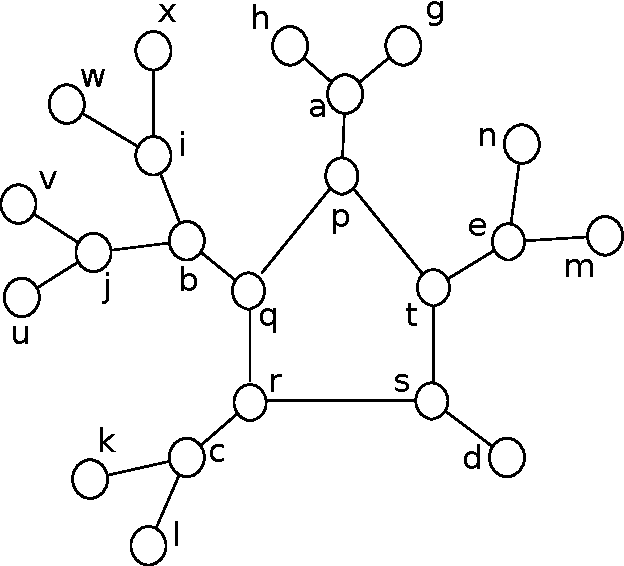
\includegraphics[scale=0.4]{pent} 
\caption{Pentagon $pqrst$}
\label{fig:pent}
\end{center}
\end{figure}

\lipsum[1]

\section{SECTION NAME}
\lipsum[2]

\begin{table}
\centering
\begin{tabular}{| c | c |}
\hline
{\bf item 1} & {\bf item 2} \\ \hline
%
abcde & 5 \\ \hline
%
pqrst & 4 \\ \hline
\end{tabular}
\caption{A sample table}
\label{table:1}
\end{table}